\scanpage{27}
% Étiquette imprimée, oblique et à l'envers sur le feuillet.
\begin{flushleft}
MISTER PROFESSOR GROTHENDIECK ALEXANDER\\
MATHEMATICS\hfill 5
\end{flushleft}

\diagram{\begin{tikzcd}[ampersand replacement=\&,column sep=huge]
\mathbb D'_3 \arrow[r] \& \mathbb D_3
\end{tikzcd}}

\margin{\figure{\begin{tikzpicture}[x=1cm,y=1cm]
\draw (0,0) .. controls (.1,.14) and (.25,.13) .. (.48,.03);
\end{tikzpicture}}}

\diagram{\begin{tikzcd}[ampersand replacement=\&,column sep=large,row sep=large]
PM_{11}(2^{\sim})\overset{?}{\simeq}PU_{0,3}
  \arrow[r,very thick] \arrow[d,leftrightarrow]
\& PM_{11}(2)\simeq TU_{0,3} \arrow[d]\\
U_{0,3}\simeq M_{11}(\unsure{\widetilde{2}^{\sim}|2^{\sim}})
  \arrow[r,very thick]
\& \begin{gathered}(U_{0,3},\{1,\omega\})\\[-2pt]{}\simeq M_{11}(\unsure{2})\end{gathered}
\arrow[ul,phantom,"\mathrm{cart}" description]
\end{tikzcd}}

\[
\deleted{\unsure{x}\longrightarrow\unsure{x^2\wedge\omega_0}}
\]
\[
\unsure{H^1}(TU_{03},\mathbb D_3;\mu_2)
\]

\diagram{\begin{tikzcd}[ampersand replacement=\&,column sep=small,row sep=large]
M_{11}(2^{\sim}) \arrow[rr]
  \arrow[dr,"{\deleted{\unsure{\mathcal D/\Pi_{0,3}|\mathbb Z/2\,\Pi_{0,3}}}}"']
\& \& M_{11}(2)\unsure{-|'} \arrow[dl] \arrow[d,leftrightarrow] \& \phantom{M}\\
\& M_{11} \arrow[d] \& M_{11}(2)' \arrow[dl] \& \\
\phantom{M}\arrow[rrruu,dashed,no head,shorten <=-10pt,shorten >=-10pt]
\& M'_{11} \& \&
\end{tikzcd}}

\diagram{\begin{tikzcd}[ampersand replacement=\&,column sep=small,row sep=large]
U_{03} \arrow[rr,"{\{1,\omega\}}"] \arrow[dr,"{\mathbb D'_3}"']
\& \& (U_{0,3},\{1,\omega\}) \arrow[dl,"{\mathbb D_3}"'] \arrow[d,"{\unsure{\mathrm{gerbe}}}"] \& \phantom{U}\\
\& (U_{0,3},\mathbb D'_3) \arrow[d,"{\unsure{\mathrm{gerbe}}}"']
\& (U_{03}) \arrow[dl,"{\mathbb D_3}"] \& \\
\phantom{U}\arrow[rrruu,dashed,no head,shorten <=-12pt,shorten >=-12pt]
\& (U_{0,3},\mathbb D_3) \& \&
\end{tikzcd}}

\diagram{\begin{tikzcd}[ampersand replacement=\&,column sep=small,row sep=large]
\begin{gathered}(\mathcal D,\Pi_{03})\\[-2pt]{}\simeq\mathcal D/\Pi_{03}\end{gathered}
 \arrow[rr,very thick,"{\mathrm{gal}}","{\{1,\omega\}}"']
 \arrow[dr,"{\begin{gathered}\mathrm{gal}\\\mathbb D'_3\end{gathered}}"']
\& \& (\mathcal D,\Pi_{03}\times\{1,\omega\})
 \arrow[dl,"{\begin{gathered}\mathrm{gal}\\\mathbb D_3\ \deleted{\unsure{\{1,\omega\}}}\end{gathered}}"']
 \arrow[d,"{\unsure{2\text{-}\uline{\mathrm{gerbe}}}}"] \& \phantom{D}\\
\& (\mathcal D,\unsure{\mathrm{Sl}(2,\mathbb Z)})
 \arrow[d,"{\unsure{2\text{-}\mathrm{gerbe}}}"']
\& (\mathcal D,\Pi_{03}) \arrow[dl,"{\begin{gathered}\mathrm{gal}\\\mathbb D_3\end{gathered}}"] \& \\
\phantom{D}\arrow[rrruu,dashed,no head,shorten <=-12pt,shorten >=-12pt]
\& (\mathcal D,\unsure{\mathrm{Sl}(2,\mathbb Z)}') \& \&
\end{tikzcd}}

\margin{26}

\scanpage{28}
% not manuscript: avis dactylographié, à l’envers, de soutenance d’une thèse de doctorat de 3ème cycle, « Algèbres de Rees », YOON Suk-Im, Montpellier, le 26 février 1982 ; soutenance prévue le 4 MARS 1982 à 15h.
\margin{27}

\scanpage{29}

\deleted{\diagram{\begin{tikzcd}[ampersand replacement=\&,column sep=small,row sep=large]
\& \& {}\arrow[r,"{\unsure{''|1}}"]
\& \mathrm{Sl}(2,\mathbb Z)\arrow[r]\arrow[d]
\& \Pi_{0,3}^{D}\arrow[d] \& \\
\& \unsure{\widetilde\varepsilon|\widetilde E}\arrow[rr]
  \arrow[ddl]\arrow[dr,dashed]
\& \& \mathbb D_3\mathop{\times}\limits_{\mathbb Z/2\mathbb Z}
       \mathbb Z/\unsure{12}\mathbb Z
       \simeq\mathbb D'_3\mathop{\times}\limits_{\mathbb Z/\unsure{2}\mathbb Z}
       \mathbb Z/6\mathbb Z
       \arrow[r]\arrow[dd,very thick]\arrow[d,dashed]
\& \mathbb D_3\mathop{\times}\limits_{\mathbb Z/2\mathbb Z}
       \mathbb Z/6\mathbb Z=\unsure{\varepsilon|E}
       \arrow[dd]\arrow[dr] \& \\
\& \& \mathbb Z\arrow[r,no head]\arrow[ddl,dashed,leftrightarrow,very thick]
\& \mathbb Z/12\mathbb Z\arrow[rr,dashed,"{\mathrm{can}}"]
       \arrow[dd,dashed,"{\mathrm{can}}"'{pos=.2}]
\& \& \mathbb Z/6\mathbb Z\arrow[ddl,"{\mathrm{can}}"]\\
\unsure{\widetilde{\mathbb D}_3^{*}|\widetilde{\mathbb D}'_3}
 \arrow[rrr,very thick]\arrow[dr]
\& \& \& \mathbb D'_3\arrow[r,very thick]\arrow[d,very thick]
\& \mathbb D_3\arrow[d,"{\mathrm{can}}"] \& \\
\& \mathbb Z\arrow[rr] \& \& \mathbb Z/4\mathbb Z\arrow[r,"{\mathrm{can}}"]
\& \mathbb Z/2\mathbb Z \&
\end{tikzcd}}}

\figure{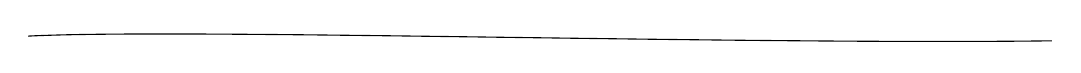
\begin{tikzpicture}[x=1cm,y=1cm]
\draw (0,.06) .. controls (2,.16) and (9,-.05) .. (13,0);
\end{tikzpicture}}

\diagram{\begin{tikzcd}[ampersand replacement=\&,column sep=small,row sep=large]
\unsure{\mathbb Z_{(\omega/2)}}\arrow[r]\arrow[d,very thick]
\& \widetilde\Pi_{0,3}^{\unsure{\circ}}
   \deleted{\unsure{\widetilde\Pi_{0,3}}}\arrow[rr,very thick]\arrow[d]
\& \& \Pi_{0,3}\arrow[d,leftrightarrow,bend left=12]
\& \& \& \\
\mathbb Z_{(\omega)}\arrow[r,very thick]\arrow[d,equal]
\& \widetilde\Pi_{0,3}^{\unsure{'}}\arrow[rr]\arrow[d,very thick]
\& \& \Pi'_{0,3}=\Pi_{0,3}\times\{1,\omega\}
   \arrow[rr]\arrow[d,bend right=12]
\& \& \Pi_{03}\arrow[d,bend right=18] \& \\
\mathbb Z\arrow[r,very thick]\arrow[d,equal]
\& \widetilde{\mathrm{Sl}}(2,\mathbb Z)=\widetilde\Pi_{0,3}^{D}
   \arrow[rr]\arrow[d]
\& \& \mathrm{Sl}(2,\mathbb Z)\arrow[rr]\arrow[d,very thick]\arrow[ddr]
\& \& \Pi_{0,3}^{D}\arrow[d]\arrow[ddr] \& \\
\mathbb Z\arrow[r]\arrow[dd,equal]
\& \widetilde{\mathbb D}_3\arrow[rr]\arrow[dd]
\& \& \begin{gathered}\mathbb D'''_3\\\margin{3}\end{gathered}\arrow[rr,"2"]\arrow[dr,"3"']\arrow[dd,"3"']
\& \& \begin{gathered}\mathbb D''_3\\\margin{\unsure{12|10}}\end{gathered}\arrow[dr,"3"]\arrow[dd,"3"'{pos=.72}] \& \\
\& \& \& \& \mathbb D'_3\arrow[rr,"2"{pos=.75}]\arrow[dd,"3"{pos=.77}]
\& \& \mathbb D_3\arrow[dd,"3"]\\
\mathbb Z\arrow[r,"12"]
\& \mathbb Z\arrow[rr]
\& \& \mathbb Z/12\mathbb Z\arrow[rr,leftrightarrow,"2"]\arrow[dr,"3"']
\& \& \mathbb Z/6\mathbb Z\arrow[dr,"3"] \& \\
\& \& \& \& \mathbb Z/4\mathbb Z\arrow[rr,"2"] \& \& \mathbb Z/2\mathbb Z
\end{tikzcd}}
\margin{\unsure{bottom|good}}

\diagram{\begin{tikzcd}[ampersand replacement=\&,column sep=large,row sep=large]
1\arrow[r,no head]
\& \mathbb Z\arrow[r,no head]\arrow[d,very thick,"{\begin{gathered}4\\\unsure{4}\end{gathered}}"]
\& \widetilde\Pi_{0,3}^{D}\arrow[r,no head]\arrow[d,no head]
\& \Pi_{0,3}^{D}\arrow[r]\arrow[d,no head]
\& 1\\
1\arrow[r,no head]
\& \mathbb Z\arrow[r,no head]
\& \widetilde\Pi_{0,3}^{D}(4)\arrow[r]
\& \Pi_{0,3}^{D}\arrow[r,very thick]
\& 1
\end{tikzcd}}

\figure{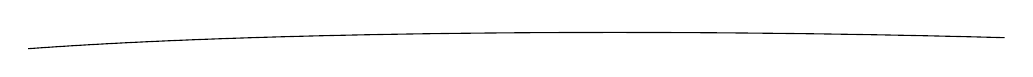
\begin{tikzpicture}[x=1cm,y=1cm]
\draw (0,0) .. controls (3,.22) and (8,.26) .. (12.4,.14);
\end{tikzpicture}}

\diagram{\begin{tikzcd}[ampersand replacement=\&,column sep=large,row sep=large]
\& \& \widetilde\Pi_{0,3}^{D}
\& \Pi_{0,3}^{D}\arrow[r,no head] \& 1\\
1\arrow[r]
\& \overset{\omega}{\mathbb Z}\arrow[r]
\& \widetilde\Pi_{0,3}^{D}(4)\arrow[r]
\& \Pi_{0,3}^{D}\times\mathbb Z/4\mathbb Z\arrow[u]\arrow[r,no head]
\& 1\\
1\arrow[r,no head]
\& \mathbb Z\arrow[r]
\& ?\arrow[r]
\& \unsure{\mathrm{Sl}(2,\mathbb Z)}\arrow[u]\arrow[r,no head]
\& 1
\end{tikzcd}}

\margin{28}

\scanpage{30}
% Secteur supérieur : un long trait courbe au crayon, terminé en crochet, descend de « par les e_i-e_j » vers le bas à gauche ;
% il traverse les trois premières lignes, la suite Z — Π̃_03 — Π_03 → 1 et la formule V(ω) ≃ V, barrées ici en bloc.
\deleted{
$V_J\deleted{\unsure{\simeq}}\inserted{=\unsure{\Gamma(X,\uline{\mathcal O}(1))}}
\deleted{e_i-e_j}$ \unsure{generated} by the $e_i-e_j$

\deleted{$\unsure{\Pi(e_i-e_j)|P(e_i-e_j)}$}
\unsure{how} \unsure{are} these \unsure{sections}
\unsure{permuted} among themselves
}

\figure{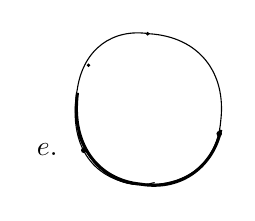
\begin{tikzpicture}[x=1cm,y=1cm]
\draw (0,.95) .. controls (.64,.91) and (.98,.45) .. (.91,-.15)
 .. controls (.86,-.78) and (.36,-1.04) .. (-.25,-.95)
 .. controls (-.83,-.83) and (-1.02,-.33) .. (-.91,.26)
 .. controls (-.83,.76) and (-.46,1.02) .. (0,.95);
\draw[line width=1.1pt] (-.91,.2) .. controls (-1,-.48) and (-.63,-.91) .. (-.11,-.96)
 .. controls (.43,-1.05) and (.82,-.71) .. (.91,-.27);
\draw (-.9,-.33) .. controls (-.72,-.82) and (-.31,-1.05) .. (.07,-.94);
\fill (-.02,.95) circle (.025);
\fill (-.77,.55) circle (.024);
\fill (-.83,-.53) circle (.035);
\fill (.89,-.32) circle (.035);
\node[left] at (-1.04,-.52) {$e.$};
\end{tikzpicture}}

\[
\deleted{e_i-e_j\qquad\unsure{\mathcal O(6)|\mathcal O(1)}}
\qquad e_i-e_j=
\]
\[
\unsure{\xi_i}.
\]

\diagram{\begin{tikzcd}[ampersand replacement=\&,column sep=small,row sep=small]
\unsure{\uline{\mathcal O}_x(1)|\uline{\mathcal O}_a(1)}\arrow[d,phantom,"{\unsure{\in}}"{description,rotate=90}]
 \& {}\ni\xi_{ij}(x)\\
\lambda \& \lambda^6=\displaystyle\prod_{i,j}\xi_{ij}(x)
\end{tikzcd}}

\deleted{\diagram{\begin{tikzcd}[ampersand replacement=\&,column sep=large]
\mathbb Z\arrow[r,no head]
\& \widetilde\Pi_{\unsure{03}}\arrow[r]
\& \Pi_{03}^{\unsure{\sharp|\ast}}\arrow[r,very thick]
\& 1
\end{tikzcd}}}

\[
(e_i-e_j)(\uline{\unsure{Q_n|Q_k}})
\qquad\deleted{\unsure{e_i-e_j}}
\]

\[
\deleted{\mathbf V(\omega)\overset{!!}{\simeq}\mathbf V}
\qquad \varphi\in V
\qquad e_i-e_j(\deleted{\unsure{Q_k}}\,
\]
\[
e_i-e_j\bmod L_{Q_k}
\]

\diagram{\(\begin{array}{ccc}
\frac12 & \frac12 & 1\\
-\frac12 & -\frac12 & -1
\end{array}\)}
\[
\left(\frac12\right)^4\qquad\sqrt[3]{\frac12}
\]

% Secteur inférieur, écrit à l'envers par rapport au secteur précédent.
\deleted{
We have seen that an orientation of a combinatorial
\inserted{\unsure{cellular|cellulation}} \deleted{\unsure{surface}}\inserted{\unsure{map}} $A$
\unsure{gives} rise \unsure{to|:} two \unsure{operators|operations}
$\vec\rho_s,\vec\rho_f$ on $\vec A$, \unsure{satisfying}
\[
\vec\rho_s^{-1}\vec\rho_f=\sigma
\]

If we take the opposite orientation, \unsure{what|what} are the
\unsure{corresponding|corresponding} \unsure{operators|operations}
$\vec\rho'_s,\vec\rho'_f$ ?
If $\vec a\in\vec A$ \unsure{comes} from $a\in A^L_+$,
it \unsure{comes} from $\sigma_na\in A^L_-$, and we have
\[
\rho_s(\sigma_na)
 =\sigma_n
   (\underbrace{\sigma_n\rho_s\sigma_n}
     _{\sigma_n\varepsilon=\rho_s^{-1}}a)
 =\sigma_n(\rho_s^{-1}a)\,-
\]
\unsure{thus} the class in $\vec A\simeq A^L/\sigma_n$
is that of $\rho_s^{-1}a$,
i.e. $\vec\rho_s^{-1}\vec a$.
\deleted{\unsure{A}}nd we therefore have
\[
\deleted{\rho_f(\sigma_na)
 =\sigma_n
  (\underbrace{\sigma_n\rho_f\sigma_n}
   _{\sigma_n\varepsilon\sigma}a)}
\]
\[
\vec\rho'_s=\vec\rho_s^{-1}
\]
hence
\[
\vec\rho'_f=\vec\rho'_s\sigma
 =\vec\rho_s^{-1}\sigma
 =\sigma\vec\rho_f^{-1}\sigma
 =\mathrm{int}(\sigma)\vec\rho_f^{-1}
\]
(This is not so \unsure{pleasant}.)
}

\margin{
% Notes perpendiculaires dans la marge droite du secteur inférieur redressé.
\[
\unsure{\widetilde Q_m|\widetilde R_m}
 -\unsure{\widetilde Q_j|\widetilde R_j}
\]
\[
\deleted{\unsure{\xi}}\quad\unsure{\gamma_h\ i\gamma_h}
\]
\[
e_j-e_i\quad -(e_i-e_h)
\]
}

\margin{29}

\scanpage{31}

\deleted{\diagram{\begin{tikzcd}[ampersand replacement=\&,column sep=large,row sep=large]
1\arrow[r,hook]
\& \mathbb Z\arrow[r,no head]
\& \widetilde\Pi\arrow[r]
\& \Pi\arrow[r,no head]\arrow[d]
\& 1\\
\& \& \& \deleted{\unsure{D''_3}} \&
\end{tikzcd}}}

\diagram{\begin{tikzcd}[ampersand replacement=\&,column sep=small,row sep=large]
\& \& \Pi_0\arrow[rr,equal]\arrow[dr]
\& \& \Pi_0\unsure{.}\arrow[dr] \& \& \\
\mathbb Z\arrow[r]\arrow[d,equal]
\& \widetilde\Pi\arrow[rr]\arrow[d]
\& \& \Pi'\arrow[rr]\arrow[d]\arrow[ddr]
\& \& \Pi\arrow[d]\arrow[ddr] \& \\
\mathbb Z\arrow[r]\arrow[dd,equal]
\& \widetilde D_{\unsure{3|0}}\arrow[rr,no head]\arrow[dd]
\& \& D'''_3\arrow[rr]\arrow[dr,no head]\arrow[dd]
\& \& D''_3\arrow[dr,very thick]\arrow[dd] \& \\
\& \& \& \& D'_3\arrow[rr,very thick]\arrow[dd,no head]
\& \& D_3\arrow[dd]\\
\mathbb Z\arrow[r,no head,"12"]
\& \mathbb Z\arrow[rr]
\& \& \mathbb Z/12\mathbb Z\arrow[rr]\arrow[dr,no head]
\& \& \mathbb Z/6\mathbb Z\arrow[dr,very thick] \& \\
\& \& \& \& \mathbb Z/4\mathbb Z\arrow[rr,no head]
\& \& \mathbb Z/2\mathbb Z
\end{tikzcd}}

\diagram{\begin{tikzcd}[ampersand replacement=\&,column sep=large,row sep=large]
\& \& \& \Pi_0\arrow[dd] \& \& \\
\& \& \deleted{\unsure{\widetilde\Pi}}\ \mathbb Z\arrow[r,very thick]
\& {} \& \& \\
1\arrow[r]
\& \mathbb Z\arrow[r]
\& \widetilde\Pi(4)\arrow[r]
\& \Pi\times\mathbb Z/4\mathbb Z\arrow[r,no head]\arrow[ddr,bend left=12]
  \arrow[dd]
\& 1 \& \\
\& \& \& \& \& \\
\& \& \& \deleted{\unsure{D_3}\times\mathbb Z/4\mathbb Z}\arrow[d]
\& D_3\times\mathbb Z/4\mathbb Z \& \\
\& \& \& 1
\& D'_3\arrow[u,phantom,"{\subset}"{description,rotate=90}] \&
\end{tikzcd}}

\diagram{\begin{tikzcd}[ampersand replacement=\&,column sep=large,row sep=large]
1\arrow[r,no head]
\& \Pi_0\arrow[r]
\& \Pi\times\mathbb Z/4\mathbb Z\arrow[r]
\& D_3\times\mathbb Z/4\mathbb Z\arrow[r]
\& 1\\
1\arrow[r,no head]
\& \Pi_0\arrow[u,equal]\arrow[r]
\& \Pi'\arrow[u,hook,very thick]\arrow[r,very thick]
\& D'_3\arrow[u,hook]\arrow[r,no head]
\& 1
\end{tikzcd}}

\[
\Pi'\subset\joinrel\relbar\joinrel\relbar\ \Pi
\]
\[
\deleted{\unsure{\widetilde\Pi}\times\unsure{\mathbb Z/4|\mathbb Z/4\mathbb Z}}
\]
\diagram{\begin{tikzcd}[ampersand replacement=\&,column sep=large]
\widetilde\Pi(4)\arrow[r]
\& \Pi\times\mathbb Z/4\mathbb Z
\end{tikzcd}}

\margin{30}